\documentclass[conference]{IEEEtran}
\IEEEoverridecommandlockouts
% The preceding line is only needed to identify funding in the first footnote. If that is unneeded, please comment it out.
\usepackage{cite}
\usepackage{amsmath,amssymb,amsfonts}
\usepackage{algorithmic}
\usepackage{graphicx}
\usepackage{textcomp}
\usepackage{subfigure}


\def\BibTeX{{\rm B\kern-.05em{\sc i\kern-.025em b}\kern-.08em
    T\kern-.1667em\lower.7ex\hbox{E}\kern-.125emX}}
\begin{document}

\title{EEE 5502 Foundation of Diginal Signal Processing\\ Literature Review\\
%{\footnotesize \textsuperscript{*}}
}

\author{\IEEEauthorblockN{Hudanyun Sheng}
\IEEEauthorblockA{\textit{Electrical and Computer Engineering} \\
\textit{University of Florida}\\
Gainesville, United States \\
hdysheng@ufl.edu}
}

\maketitle

\begin{abstract}
Representation, analysis and processing of large datasets on graphs has attracted much interests, with the fact that graphs are thought and proven to be able to encode complex geometric structures. Examples of graph signals including social and economic networks, transportation networks, molecular and gene regulatory networks. Although a signal on a graph with N vertices and a classical discrete-time signal with N samples can be viewed as vectors and are thought to be sharing similarities, the truth that processing the graph signal in the classical way of processing discrete-time signal ignores the key dependencies arising from the irregular data domain becomes the main obstacle to the usage of classical signal processing techniques in the graph setting. Here we have reviewed the challenges of processing signals on graphs, and learned that algebraic and spectral graph theoretic concepts together with computational harmonic analysis are used to address those challenges, which is the emerging field of signal processing on graphs. The spectral graph theory is reviewed with basic graph theories, including the graph Laplacian, the graph Fourier transform, and most importantly, the generalized operators for signals on graphs. Graph Fourier transform, one of the operators, is further studied. It is demonstrated that the graph signals can be sparsely represented in their frequency domain, and the graph signals is a natural extension of the classical time-series DSP theory, with the potential application as efficiently representing structured data with sparseness. 
\end{abstract}

\begin{IEEEkeywords}
DSP, Graph signals, graph Laplacian, discrete Fourier transform, graph Fourier transform
\end{IEEEkeywords}

\section{Introduction}
The real world data, such as the social network data, the temperature data, the traffic data are often structured, and when analyzing them, it is better if the structure behind the data are taken into account. Graphs are appealing tools and are considered as generic data representation forms which are useful especially when aiming to describe the geometric structures of data, also an efficient method when processing high-dimensional data, for the fact that graphs have efficient representations for pairwise relations between entities. An example of a graph signal is shown in Figure \ref{1}. Both a signal on a graph with N vertices and a classical discrete-time signal with N samples can be viewed as N-dimensional vectors\cite{b1}. However, the fact that processing the graph signal using the same ways as a discrete-time signal discarding the key dependencies arising from the irregular data domain hinder the application of the classical signal processing techniques in the graph setting. Examples of challenges include: 1) being not quite meaningful when trying to have similar definition of graph signal translation; 2)being nontrivial to define an operator which correspond to translation in the spectral domain as in classical Fourier transform; 3)being unable to define downsampling for graph signals; etc. These challenges result from the fact that the the graphs having  irregular structures. To face with these challenges, researches have been done and the main approaches can be categorized into two main areas: vertex domain analysis which is analogous to spatial domain analysis and frequency domain analysis which analogous to graph spectral domain analysis. 
\begin{figure}[!htbp]
\centerline{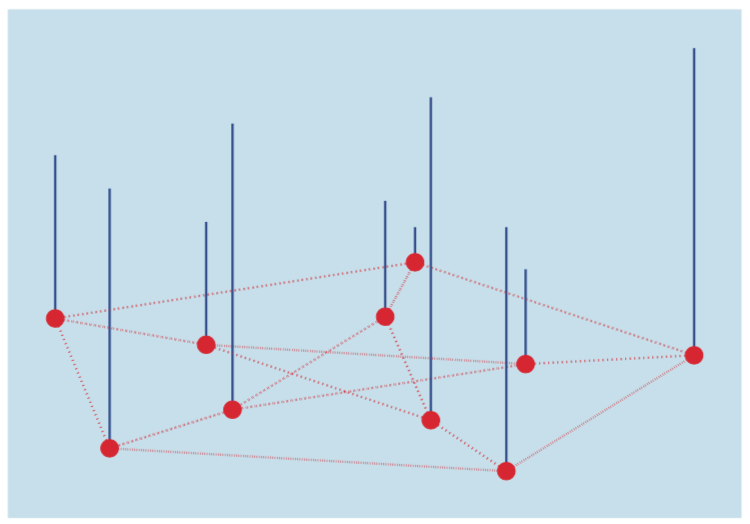
\includegraphics[width=3.4in]{1.png}}
\caption{A random positive graph signal on the vertices of the Petersen graph. The height of each blue bar represents the signal value at the vertex. Image courtesy of \cite{b1}.}
\label{1}
\end{figure}

\section{Summary of articles}
Analyzing signal defined on an undirected, connected, weighted graph $G=\{\nu, E, W\}$ first attracted attention. Basic definitions of spectral graph theory are reviewed.The weighted graph consists of a finite set of vertices $\nu$, a set of edges $E$ and a weighted adjacency matrix $W$. Assuming an edge $e=(i,j)$ connects vertices $i$ and $j$, $W_{ij}$ represents the weight of the edge. If there is no edge connecting vertices $i$ and $j$, $W_{ij}=0$. A signal or function $f:\nu\to R$ defined on the vertices of the graph can be represented as a vector $f\in R^N$, where the $i$th component of the vector f represents the function value at the $i$th vertex in $\nu$. An example of graph representations for standard DSP signals is shown in the figure \ref{5}\\
\begin{figure}[htbp]
\centerline{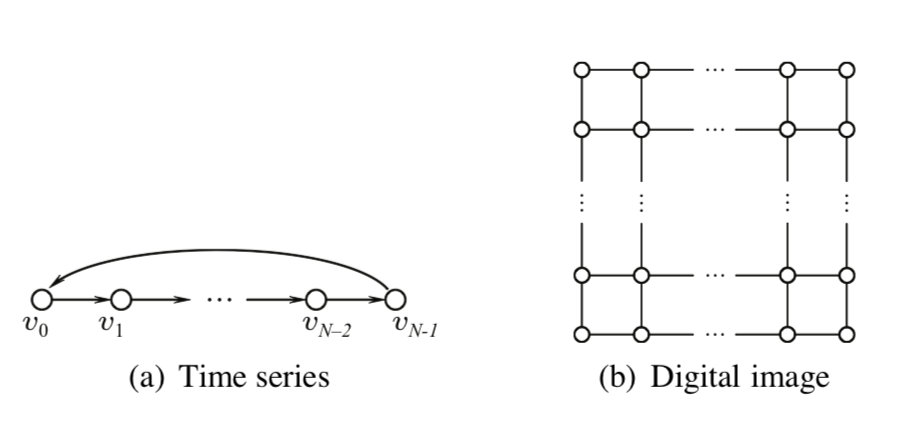
\includegraphics[width=3.4in]{5.png}}
\caption{Graph representations for standard DSP signals. Image courtesy of \cite{b4}.}
\label{5}
\end{figure}

The generalized operators for signals on graphs are also reviewed and discussed, each operator is defined on both the vertex and the graph spectral domain. 
\begin{enumerate}
\item Shift. In classical digital signal processing, time delay also known as time shift, denoted by $z^{-1}$ is considered the basic building block for filters. With the graph representation of the standard DSP signals, taking the one in figure \ref{5} as example, the adjacency matrix of which can be represented as an $N\times N$ circulant  matrix $A$ with weights. Thus the shift can be represented as $\tilde{s} = As$. The graph shift is thus defined as 
$$\tilde{s}_n = \sum_{m=0}^{N-1}A_{n,m}s_m=\sum_{m\in\mathcal{N}_n}A_{n,m}s_m$$
\item Filtering. 
\begin{itemize}
\item Frequency filtering: similar to the definition of filtering the frequency domain for classical discrete signals $\hat{f}_{out}(\xi)=\hat{f}_{in}(\xi)\hat{h}(\xi)$, the definition of graph spectral filtering is defined as
$$\hat{f}_{out}(\lambda_l)=\hat{f}_{in}(\lambda_l)\hat{h}(\lambda_l)$$

\item Filtering in the vertex domain: the definition of filtering a graph in the vertex is intuitively given by combine the components of input signal at vertices within a K-hop neighborhood
$$f_{out}(i)=b_{i,j}f_{in}(i)+\sum_{j\in\mathcal{N}(i,K)}b_{i,j}f_{in}(j)$$
\end{itemize}
Relating filtering in the graph spectral domain to filtering in the vertex domain, a highly useful property relating the smoothness of a filtering kernel to the localization of filtered signals is stated: when the frequency filter is an order $K$ polynomial, the frequency filtered at vertex $i$ is a linear combination of the components of the input signal at vertices within a K-hop local neighborhood of vertex $i$. \\
One application of graph filter is proposed in \cite{b4} where the graph filters are used for data classification. In the proposed method, the classification system is interpreted as a graph filter. The matrix $A$ represents the edge weights, with  edge weights $A_{k,m}\geq 0$ indicating similarity or dependency between nodes. A filter $h(A) = h_0\mathbf{I}+...+h_L\mathbf{A}^L$ produces the predicted labels
$$\mathbf{s}^{pred}=h(\mathbf{A})\mathbf{s}^{known}$$
And this classification method is test on the MNIST data set as an image classification problem.

\item Convolution is defined with the graph Laplacian eigenvectors
$$(f*h)(i):=\sum_{l=0}^{N-1}\hat{f}(\lambda)\hat{h}(\lambda_l)u_l(i)$$

\item Translation for graph signals is rather considered as a kernelized operator, as opposed to be considered as in the vertex domain. 
$$(T_ng)(i):=\sqrt{(N)}(g*\delta_n)(i)=\sqrt N\sum_{l=0}^{N-1}\hat{g}(\lambda_l)u_l^*(n)u_l(i)$$
\end{enumerate}

The graph Laplacian is defined as $\mathcal{L}:=D-W$, $D$ is called the degree matrix, which is a diagonal matrix whose $i$th diagonal element is equal to the sum of the weights of all the edges point to vertex $i$. The graph Laplacian is a difference operator, as, for any signal $f\in \mathbb{R}^N$, it satisfies
$$(\mathcal{L}f)(i)=\sum_{j\in\mathcal{N}_i}[f(i)-f(j)]$$
where the neighborhood $\mathcal{N}_i$ is the set of vertices connected to vertex $i$ by an edge. It is also known that the Laplacian quadratic form $(f^T\mathcal{L}f)(i)=\frac{1}{2}\sum_{j\in\mathcal{N}_i}[f(i)-f(j)]^2$ is a measure of ``smoothness".\\ 
Result from the fact that the graph Laplacian $\mathcal{L}$ is a real symmetric matrix, it has a complete set of orthonormal eigenvectors, the corresponding eigenvalues are referred to as the entire spectrum of the graph Laplacian: $\sigma(\mathcal{L}):=\{\lambda_0, \lambda_1, ..., \lambda_{N-1}\}$.\\
Knowing that the Laplacian $\mathcal{L}$ admits the eigendecomposition $\mathcal{L}u_{l}=\lambda_lu_l$, analogous to the classical Fourier transform
$$\hat{f}(\xi)=\int_Rf(t)e^{-2\pi i\xi t}dt$$
which can also be expressed as the eigenfunctions of the one-dimensional Laplace operator
$$\Delta(e^{2\pi i\xi t})=-\displaystyle\frac{\partial^2}{\partial t^2}e^{2\pi i \xi t} = (2pi\xi)^2e^{2\pi i\xi t}$$
the graph Fourier transform $\hat{f}$ of functions of the vertices of $\mathcal{G}$ is defined as expansion of $f$ in terms of the eigenvectors of the graph Laplacian. 
$$\hat{f}(\lambda_{l}):=\langle f, u_l\rangle=\sum_{i=1}^Nf(i)u_l^*(i)$$
The inverse graph Fourier transform is given by
$$f(i)=\sum_{l=0}^{N-1}\hat{f}(\lambda_l)u_l(i)$$
One interesting thing here is that, the Fourier transform in the graph settings show some similar characteristics of frequency: similar to the characteristics in the classical Fourier analysis, lower frequency represents smooth functions while high frequency represents much oscillate, the graph Laplacian eigenvectors associated with low frequencies vary slowly. As it can be observed in the figure \ref{2}. Which can be explained by the analysis of eigenvectors and eigenvalues: eigenvectors associated with smaller eigenvalues have values that vary less rapidly along the edges.
\begin{figure}[htbp]
\centerline{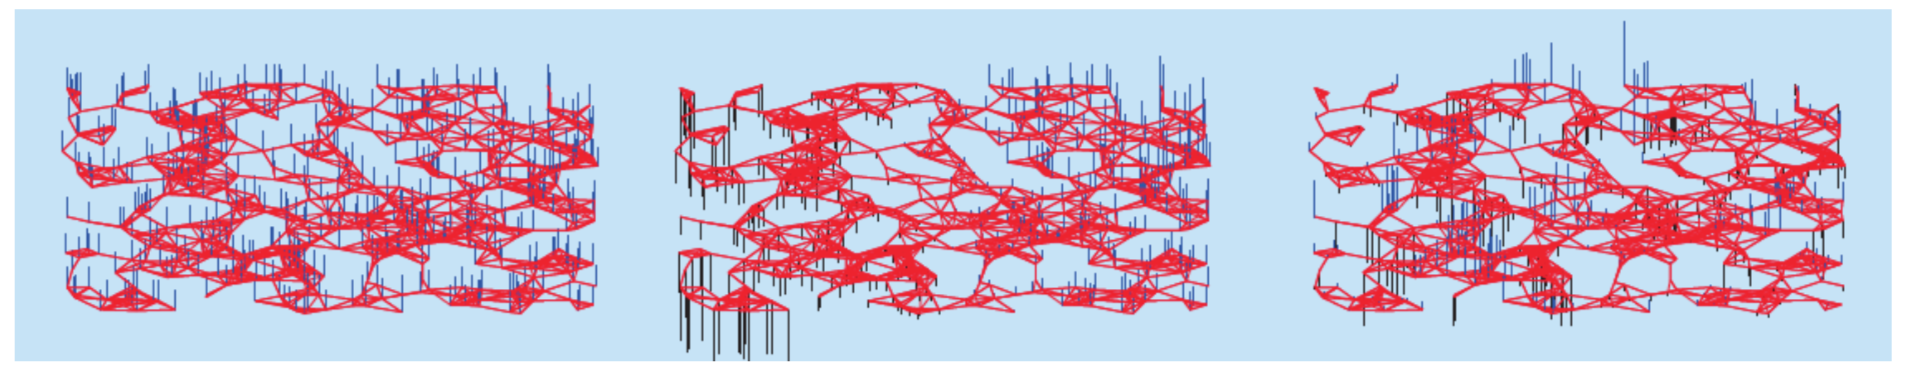
\includegraphics[width=3.5in]{2.png}}
\caption{From left to right: the graph Laplacian eigenvectors $u_0$, $u_1$, $u_{50}$ of a random network. It is observed that $u_{50}$ contains more zero crossings than the eigenvectors $u_0$ and $u_1$. Image courtesy of \cite{b1}.}
\label{2}
\end{figure}

Analogous to classical signals and Fourier transform, the signals are represented in two domains: time domain and frequency, with the graph settings, the signal can also be represented in two different domains: the vertex domain and the graph spectral domain. 
Details regrading frequency filtering is further discussed. When classical Fourier transform is considered, frequency filtering has a process like this: the Fourier transform of the original signal $\hat{f}(\omega)$ is obtained, and a filter $\hat{g}(\omega)$ is applied to the signal.When the graph Fourier transform is considered, the spectral filtering is apply filter with transfer function $\hat{g}(.)$ to a graph signal: $\hat{g}(\lambda_l)\hat{f}(\lambda_l)$. Based on the definition of the graph Laplacian and graph Fourier transform, the graph Fourier transform can also be represented as $\mathbf{u}^Tf$, where $\mathbf{u}$ are the eigenvectors of the Laplacian matrix. And filtering is thus represented as $g(\hat{\Lambda})\mathbf{u}f$, where $\hat{g}(\Lambda)$ is the diagonal matrix with transfer function value of every eigenvalues, i.e. $\hat{g}(\lambda_i)$. Thus it is concluded that the Laplacian operator filters the signal in the spectral domain by its eigenvalues. An example of graph spectral filtering is image denoising. The results using two-dimensional Gaussian low-pass filter and the one with graph filtering are compared in figure \ref{3}. From the results it is observed that the classical Gaussian filter tend to also smooth across the images edges, while the graph spectral filtering method does not smooth much across the edges, since the geometric structure of the image is encoded in the graph Laplacian.\\
\begin{figure}[htbp]
\centerline{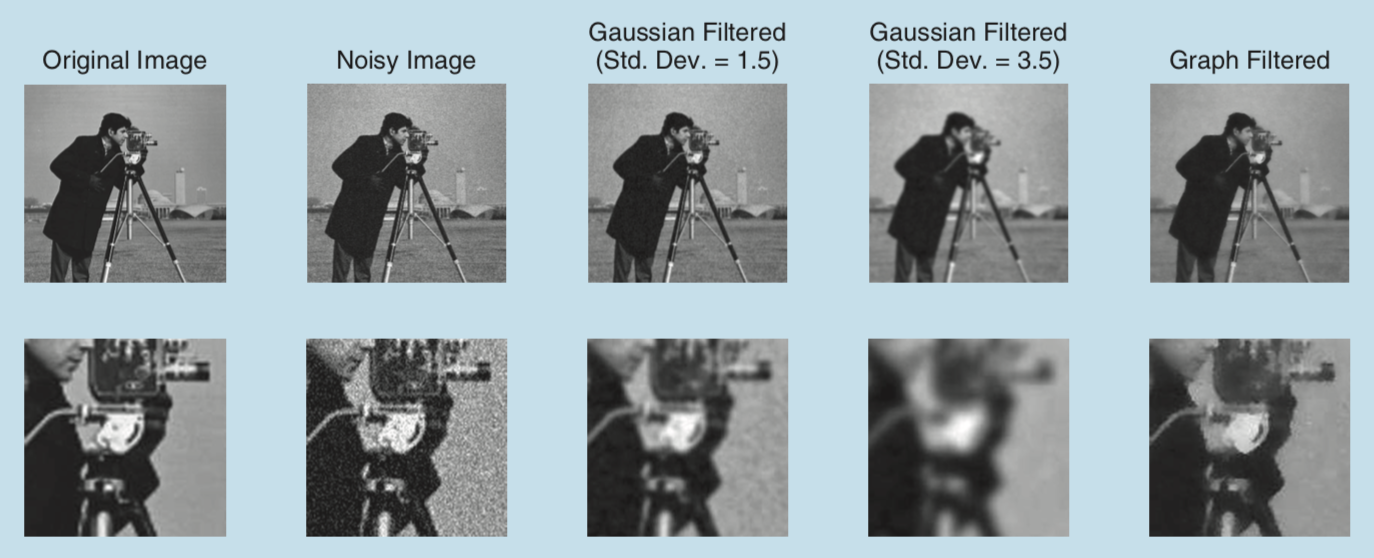
\includegraphics[width=3.5in]{3.png}}
\caption{Results of image denoising via classical Gaussian filtering and graph spectral filtering. The images in second row are zoomed-in versions of those in the first row. Image courtesy of \cite{b1}.}
\label{3}
\end{figure}

When it comes to the consideration of spatial features of the graph, the vertex domain designs is defined. The examples of spatial features including node connectivity and distances between vertices. One important branch of signal processing on graphs vertex domain is wavelets on unweighted graphs. As is known that the classical wavelet transforms are useful because of its ability of grasping information in both frequency and time (or space) domain. And classically, the locality is measured by the ``spread" of graph signals in both domains. When it comes to the graph signal, the ``spread" is heuristically defined, with the spatial spread being $\Delta_\mathcal{G}^2(f):=min_{i\in\mathcal{V}}\{\Delta_{\mathcal{G}, i}^2\}$, and the spectral spread being $\Delta_{\sigma}^2(f):=min_{\mu\in R_+}\{\displaystyle\frac{1}{||f||_2^2}\sum_{\lambda\in\sigma (\mathcal{L})}[\lambda-\sqrt{\mu}]^2[\hat{f}(\lambda)]^2\}$. Based on the definitions above, it is stated that there exists a tradeoff between spatial and spectral localization in graph wavelets. And intuitively there are two types of graph wavelet transform, i.e. vertex domain designs and graph spectral domain designs. As an example, the graph wavelet transform of Crovella and Kolaczyk (CKWT) which are wavelets based on geodesic or shortest-path distance is used as an example for the vertex domain design. And the spectral graph wavelet transform (SGWT), which contains one scaling function centered at each vertex and K wavelets centered at each vertex with scales $\{t_1, t_2, ..., t_K\}\in \mathbb{R}_+$ is used as example for the graph spectral domain design. The spatial and spectral spreads of the two graph wavelet transforms are calculated and the results are shown in figure \ref{4}. From the figure we can conclude that the SKWT wavelets are less localized spectrally and more localized spatially than the SGWT wavelets. Thus states that there exists a tradeoff between the spatial and spectral resolutions of signals defined on graphs. Some further experiments showed that the graph wavelet transforms are able to localize the high-pass information of the signal in the spatial domain.\\
\begin{figure}[htbp]
\centerline{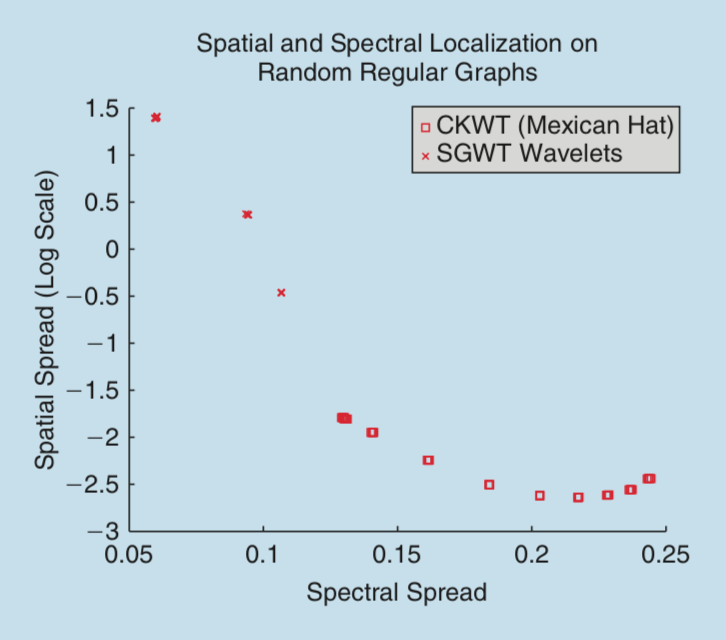
\includegraphics[width=3.5in]{4.png}}
\caption{The average spatial and spectral spreads of two example wavelet transforms. Image courtesy of \cite{b1}.}
\label{4}
\end{figure}
Spectral graph theory is considered a tool to define frequency spectra and to expand the bases for graph Fourier transforms in the area of signal processing on graphs. 

\section{Conclusions}  
With the fact that most of the real life data are structured and motivated by the need to take the structure behind the data into account when analyzing, the research question of graph signal processing is brought up. With the basic definition of graph theory, most importantly the graph Laplacian, the classical Fourier theory, the basic concepts of graph Fourier theory is defined by extension from the classic Fourier theory. The generalization of elementary operators, considered as core of graph signal processing algorithms, is also discussed. Two main areas are discussed in detail: graph spectral domain analysis and graph frequency domain analysis. Some examples are shown with the advantages of graph signal processing. These applications include denoising, semi-supervised learning, clustering, dimensionality reduction, neuroimaging, urban computing, geoscience and remote sensing, etc.\\
With all these applications and potentials, it is still a research question with a lot open issues and new potential research focuses. These issues include the construction of the underlying graph, with no prior explicit knowledge of how the construction would affect the resulting properties; it is not clear what basis to use as the graph spectral filtering basis; when it comes to extremely large graphs, it is not practical to compute the eigenvectors of the graph Laplacian; the link between structural properties of graph signals and their underlying graphs to properties of the generalized operators and transform coefficient is not understood.\\
Thus, the potential future researches can be focused on these topics: 
\begin{enumerate}
\item Mathematical models for graph signals, which learn the global and local smoothness and the underlying physical processes.
\item Graph construction which focus on the way to infer topologies given the observed data.
\item Consider the directed graphs, or time series of data on each vertex in a graph, or a time-varying series of underlying graphs, or any combination of them.
\end{enumerate}

\bibliographystyle{ieeetr}
%\bibliography{ref}
\begin{thebibliography}{00}
\bibitem{b1}D. I. Shuman, S. K. Narang, P. Frossard, A. Ortega, and P. Vandergheynst, "The emerging field of signal processing on graphs: Extending high-dimensional data analysis to networks and other irregular domains", IEEE Signal Processing Magazine, vol. 30, no. 3, pp. 83-98, 2013.
\bibitem{b2}Sandryhaila, A., Moura, J.M.F.: 'Discrete signal processing on graphs', IEEE Trains. Signal Process., 2013, 61, (7), pp. 1644-1656
\bibitem{b3}Sandryhaila, A., Moura and J.M.F.: 'Discrete Signal Processing on Graphs: Graph Fourier Transform'.
\bibitem{b4}Sandryhaila, A., Moura, J.M.F.: 'Discrete Signal Processing on Graphs: Graph Filters', IEEE International Conf. on Acoustics, Speech and Signal., 2013.
\end{thebibliography}


\end{document}
